\documentclass[8pt]{beamer}
\usepackage[utf8]{inputenc}
\usepackage{xcolor}
\usepackage{colortbl}
\usepackage{epsfig}
% \usepackage{cancel}
\usepackage{ulem}
% \usepackage{threeparttable} % Joao Pela: 
\usepackage{amsmath}
\usepackage{hyperref}
\usepackage{appendixnumberbeamer}
% \usepackage{feynmp}         % For latex produced Feynman Diagrams

% Rule for feynmp diagrams to be considered graphics
% \DeclareGraphicsRule{*}{mps}{*}{}
% 
% % New compile sequence for feynmp
% \makeatletter
% \def\endfmffile{%
%   \fmfcmd{\p@rcent\space the end.^^J%
%           end.^^J%
%           endinput;}%
%   \if@fmfio
%     \immediate\closeout\@outfmf
%   \fi
%   \ifnum\pdfshellescape=\@ne
%     \immediate\write18{mpost \thefmffile}%
%   \fi}
% \makeatother

\usetheme{Madrid}

\author[J. Pela]{João Pela}
\title{Run 2 Trigger Study}
\institute[ICL]{Imperial College London}
\date{2014-04-06}

% The log drawn in the upper right corner.
\logo{\includegraphics[height=0.115\paperheight]{img/Logo_CMSICL.png}}

\begin{document}
\setlength{\unitlength}{1mm}

% ###################################################
\begin{frame}
  \titlepage
\end{frame}

% ###################################################
\begin{frame}{Today's presentation}
 
\begin{block}{Topics}
 
\begin{itemize}
  \item L1 and HLT efficiencies for 13 $TeV$ for the 3 TSG proposed scenarios
  \item Comparison between 8 $TeV$ and 13 $TeV$ samples.
  \item Signal efficiency as a function of L1T seed threshould.
\end{itemize}
 
\end{block}

\end{frame}

% ###################################################
\begin{frame}{Samples}

For comparison we use numbers obtained by rerunning a L1+HLT menu from Run D over a 8 $TeV$ signal sample (to have all parked data trigger available):

\begin{block}{8 $TeV$ Dataset}

\resizebox{\linewidth}{!}{
\begin{tabular}{|l|c|}
\hline
Sample \\
\hline \hline
/VBF\_HToZZTo4Nu\_M-120\_8TeV-pythia6/Summer12-PU\_S9\_START52\_V9-v1/GEN-SIM-RECO \\
\hline
\end{tabular}
}

\end{block}

For the 13 $TeV$ study we will use the TSG provided samples. Note that this samples where produced using POWHEG with 
Higgs mass 125 $GeV$ while the 8 $TeV$ samples were produced using Pythia for Higgs mass of 120 $GeV$ and using a 
different PU scenario.

\begin{block}{13 $TeV$ Dataset}

\resizebox{\linewidth}{!}{
\begin{tabular}{|l|c|}
\hline
Sample & Events \\
\hline \hline
/VBF\_HToInv\_M-125\_13TeV\_powheg-pythia6/Fall13dr-tsg\_PU20bx25\_POSTLS162\_V2-v1/AODSIM & 484096 \\
/VBF\_HToInv\_M-125\_13TeV\_powheg-pythia6/Fall13dr-tsg\_PU40bx50\_POSTLS162\_V2-v1/AODSIM & 482996 \\
/VBF\_HToInv\_M-125\_13TeV\_powheg-pythia6/Fall13dr-tsg\_PU40bx25\_POSTLS162\_V2-v1/AODSIM & 483696 \\
\hline
\end{tabular}
}

\end{block}
 
\end{frame}

% ###################################################
\begin{frame}{Seeds}

Lets review our HLT paths and their corresponding seeds:

\begin{block}{HLT Paths vs. Seeds}
 
\resizebox{\linewidth}{!}{
\begin{tabular}{|l|l|}
\hline
HLT Path & Seeds \\ 
\hline \hline
HLT\_DiPFJet40PFMETnoMu65MJJ600VBFLeadingJets & L1\_ETM40 \\
HLT\_DiPFJet40PFMETnoMu65MJJ800VBFAllJets     & L1\_ETM40 \\
\hline \hline
HLT\_DiJet20\_MJJ650\_AllJets\_DEta3p5\_HT120\_VBF & L1\_HTT200 OR L1\_HTT175 OR L1\_ETM40 OR L1\_ETM50 \\
HLT\_DiJet30\_MJJ700\_AllJets\_DEta3p5\_VBF        & L1\_HTT200 OR L1\_HTT175 OR L1\_ETM40 OR L1\_ETM50 \\
HLT\_DiJet35\_MJJ650\_AllJets\_DEta3p5\_VBF        & L1\_HTT200 OR L1\_HTT175 OR L1\_HTT150 OR L1\_ETM40 \\
HLT\_DiJet35\_MJJ700\_AllJets\_DEta3p5\_VBF        & L1\_HTT200 OR L1\_HTT175 OR L1\_ETM40 \\
HLT\_DiJet35\_MJJ750\_AllJets\_DEta3p5\_VBF        & L1\_HTT200 OR L1\_HTT175 OR L1\_ETM40 \\
\hline
\end{tabular}
}

\end{block}

Even though we only use L1\_ETM seeded events parked data paths have L1\_HTT seeds too.

\end{frame}

% ###################################################
\begin{frame}{}

\begin{block}{Efficiencies}
 
\resizebox{\linewidth}{!}{
\begin{tabular}{|l|l|l|l|l|}
\hline
Trigger                                      & 8 $TeV$   & PU40bx50  & PU20bx25   & PU40bx25  \\
\hline \hline
L1\_ETM40                                     & -         & 0.526785  & 0.48077    & 0.498313  \\
\hline \hline
HLT\_DiPFJet40PFMETnoMu65MJJ600VBFLeadingJets & 0.104736  & 0.11675   & 0.107917   & 0.10923   \\
HLT\_DiPFJet40PFMETnoMu65MJJ800VBFAllJets     & 0.0766837 & 0.0919718 & 0.0849935  & 0.0878568 \\
HLT\_DiJet35MJJ650VBFAllJets                  & 0.12091   & 0.0792947 & 0.12493    & 0.119854  \\
HLT\_DiJet35MJJ700VBFAllJets                  & 0.109952  & 0.0691848 & 0.114779   & 0.10998   \\
HLT\_DiJet35MJJ750VBFAllJets                  & 0.100287  & 0.0620005 & 0.106152   & 0.102006  \\
HLT\_DiJet20MJJ650VBFAllJetsHT120             & 0.129063  & 0.105392  & 0.149766   & 0.13758   \\
HLT\_DiJet30MJJ700VBFAllJets                  & 0.120932  & 0.0775783 & 0.127966   & 0.125002  \\
\hline
\end{tabular}
}

\end{block}

\end{frame}

% ###################################################
\begin{frame}{L1T ETM}

\begin{columns}

\column[t]{0.45\linewidth}
\begin{block}{L1T ETM}
 
\centering
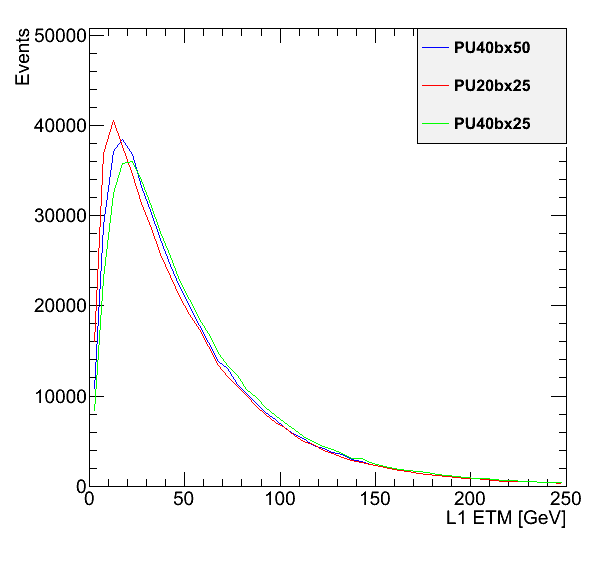
\includegraphics[width=\linewidth]{img/hL1ETM.png}
 
\end{block}

\column[t]{0.45\linewidth}
\begin{block}{Sig. Eff. vs L1T ETM}
 
\centering
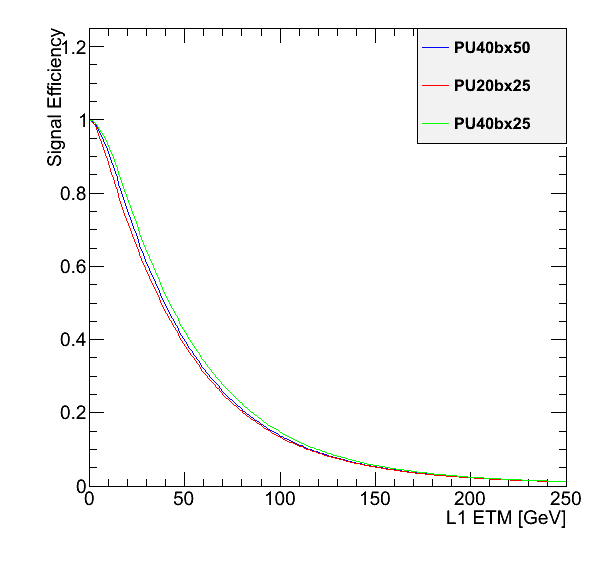
\includegraphics[width=\linewidth]{img/hEffL1ETM.png}
 
\end{block}

\end{columns}

\end{frame}

% ###################################################
\begin{frame}{L1T HTT}

\begin{columns}

\column[t]{0.45\linewidth}
\begin{block}{L1T HTT}
 
\centering
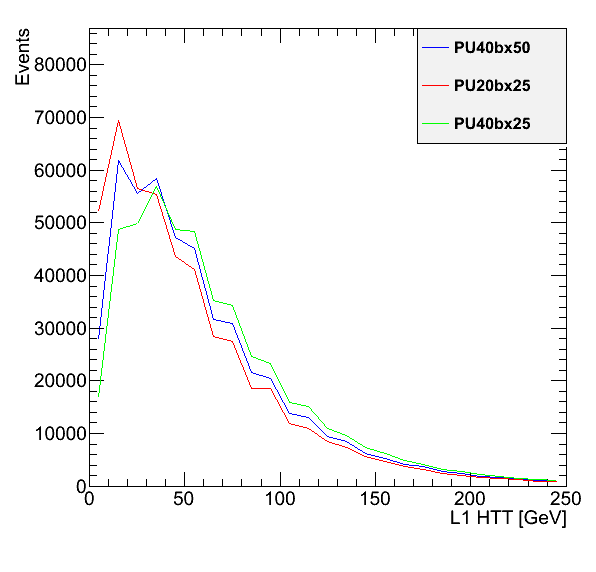
\includegraphics[width=\linewidth]{img/hL1HTT.png}
 
\end{block}

\column[t]{0.45\linewidth}
\begin{block}{Sig. Eff. vs L1T HTT}
 
\centering
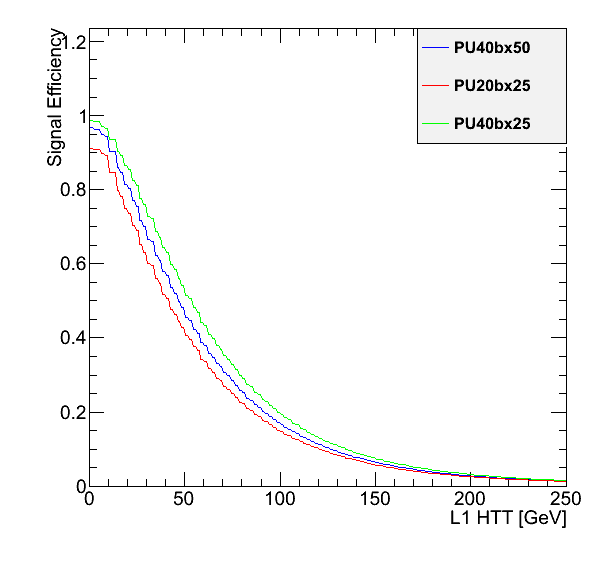
\includegraphics[width=\linewidth]{img/hEffL1HTT.png}
 
\end{block}

\end{columns}

L1 HTT is the sum of all L1 Jets and the kinks on the  plots are most likely due to two effects:
\begin{itemize}
  \item A L1 Jet seed need to have at least 5 $GeV$
  \item A L1 Jet to be included in HTT needs to have at least least 10 $GeV$. 
\end{itemize}

\end{frame}

% ###################################################
\begin{frame}{Summary and next steps}
 
\begin{block}{Summary:}
 
\begin{itemize}
  \item Our trigger when applied to 13 $TeV$ samples and various spacing and PU scenarios show some small variations on signal efficiency depending of the algorithm while compared with 8 TeV samples. 
\end{itemize}

\end{block}

\begin{block}{Next Steps:}
 
\begin{itemize}
  \item HLT study 
  \item Rerun run D HLT on 8 $TeV$ samples so we can compare samples with same generator and Higgs mass
\end{itemize}
 
\end{block}

\end{frame}

\end{document}